\subsubsection*{2D Shapes}

\textbf{Triangle}
\begin{center}
    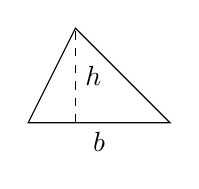
\begin{tikzpicture}[scale=0.6]
    \draw (0,0) -- (3,0) node[midway,below] {$b$} -- (1,2) -- cycle;
    \draw[dashed] (1,0) -- (1,2) node[midway,right] {$h$};
    \end{tikzpicture}
\end{center}
Area $= \frac{1}{2}bh = \sqrt{s(s-a)(s-b)(s-c)}$ \\
$s = \frac{a+b+c}{2}$

\textbf{Sector}
\begin{center}
    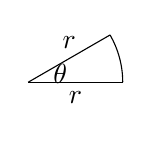
\begin{tikzpicture}[scale=0.6]
    \draw (0,0) -- (30:2) node[midway,above] {$r$};
    \draw (0,0) -- (0:2) node[midway,below] {$r$};
    \draw (0:2) arc (0:30:2);
    \node at (15:0.7) {$\theta$};
    \end{tikzpicture}
\end{center}
Area $= \frac{1}{2}r^2\theta$ (rad) $= \pi r^2 \frac{\theta}{360}$ \\
Arc $s = r\theta$ (rad)

\textbf{Polygon Area} \\
$A = \frac{1}{2} | \sum_{i=1}^{n} (x_i y_{i+1} - x_{i+1} y_i) |$

\textbf{Pick's Theorem} \\
$A = I + \frac{B}{2} - 1$ ($I$: interior, $B$: boundary)

\subsubsection*{3D Shapes}
\textbf{Sphere} \\
$V=\frac{4}{3}\pi r^3, \quad S=4\pi r^2$

\textbf{Cylinder} \\
$V=\pi r^2 h, \quad S=2\pi r(r+h)$

\textbf{Cone} \\
$V=\frac{1}{3}\pi r^2 h, \quad S=\pi r(r+\text{slant})$

\subsubsection*{Coordinate Geometry}
\textbf{Distance & Slope} \\
$d = \sqrt{\Delta x^2 + \Delta y^2}, \quad m = \frac{\Delta y}{\Delta x} = \tan \theta$

\textbf{Rotation} (CCW by $\theta$) \\
$x' = x \cos \theta - y \sin \theta$ \\
$y' = x \sin \theta + y \cos \theta$

\subsubsection*{Trigonometry}
\textbf{Sine Rule:} $\frac{a}{\sin A} = \frac{b}{\sin B} = \frac{c}{\sin C} = 2R$ \\
\textbf{Cosine Rule:} $c^2 = a^2 + b^2 - 2ab \cos C$ \\
\textbf{Area:} $\frac{1}{2}ab \sin C$

\subsubsection*{Vectors}
$|A| = \sqrt{x^2+y^2}, \quad A \cdot B = |A||B|\cos\theta$ \\
$A \times B = |A||B|\sin\theta \implies x_1y_2 - x_2y_1$
